\begin{tframe}{Autonomous Exploration}

\bigskip
\begin{tabular}{cl}
\begin{tabular}{c}
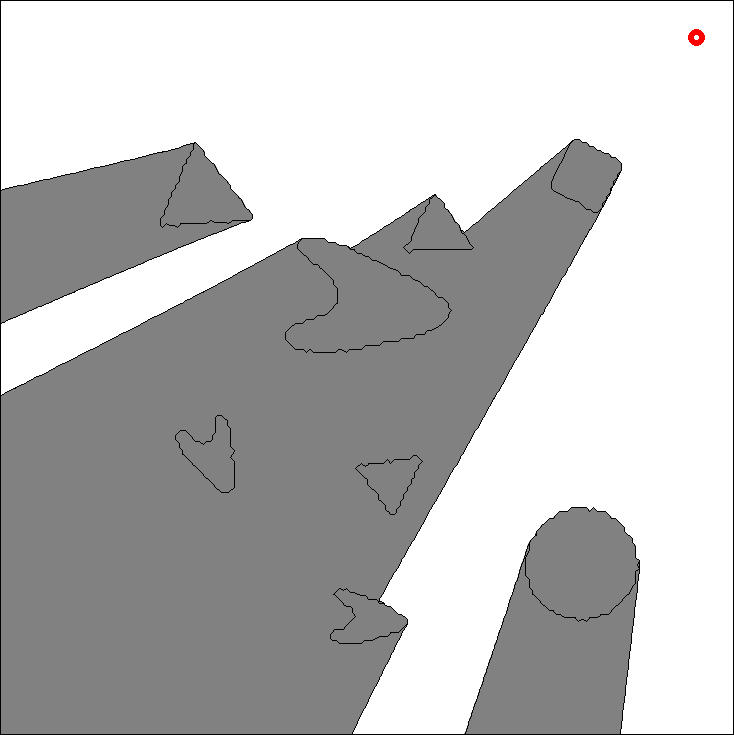
\includegraphics[width=2in]{media_exploration/2D_scene_01}
\end{tabular}
&\phantom{\parbox[t]{.5\textwidth}{
\begin{itemize}
 \item ``Frontier chasing''
 \item Heuristics
\end{itemize}}}
\end{tabular}
\end{tframe}

\addtocounter{framenumber}{-1}
\begin{tframe}{Autonomous Exploration}

\bigskip
\begin{tabular}{cl}
\begin{tabular}{c}
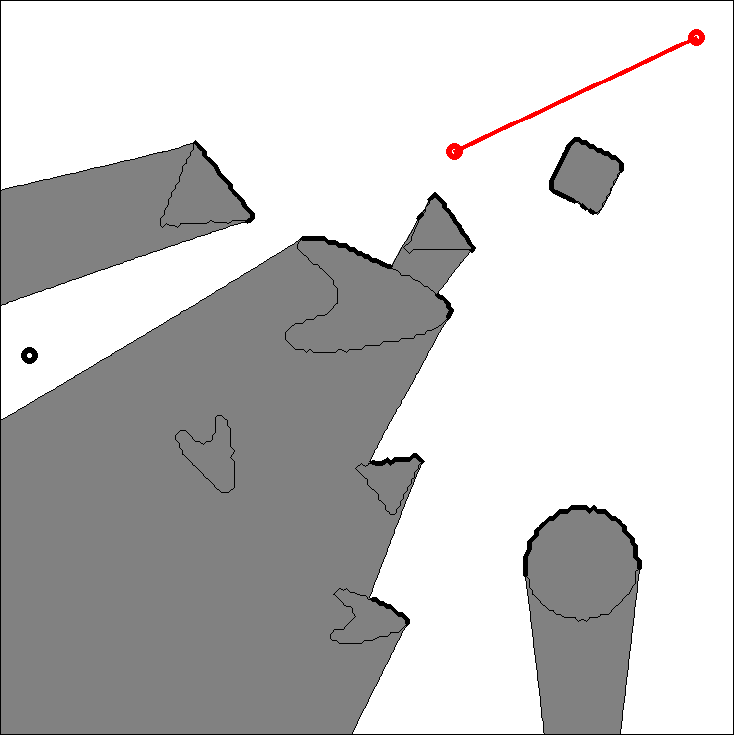
\includegraphics[width=2in]{media_exploration/2D_scene_02}
\end{tabular}
&\visible<2>{\parbox[t]{.5\textwidth}{
\begin{itemize}
 \item ``Frontier chasing''
 \item Heuristics
\end{itemize}}}
\end{tabular}
\end{tframe}


\begin{tframe}{Exploring a Random Room}
\begin{center}
\begin{tabular}{c}
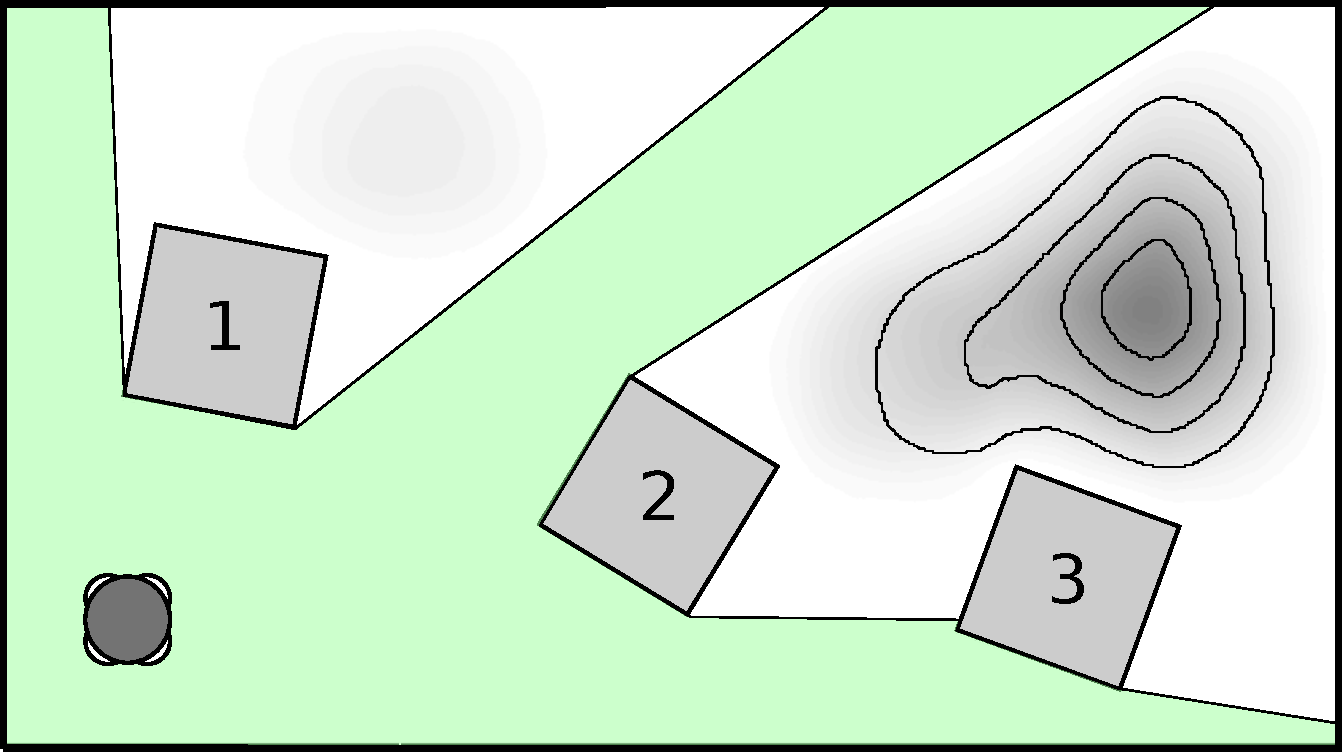
\includegraphics[height=1in]{media_exploration/random_block_marg}
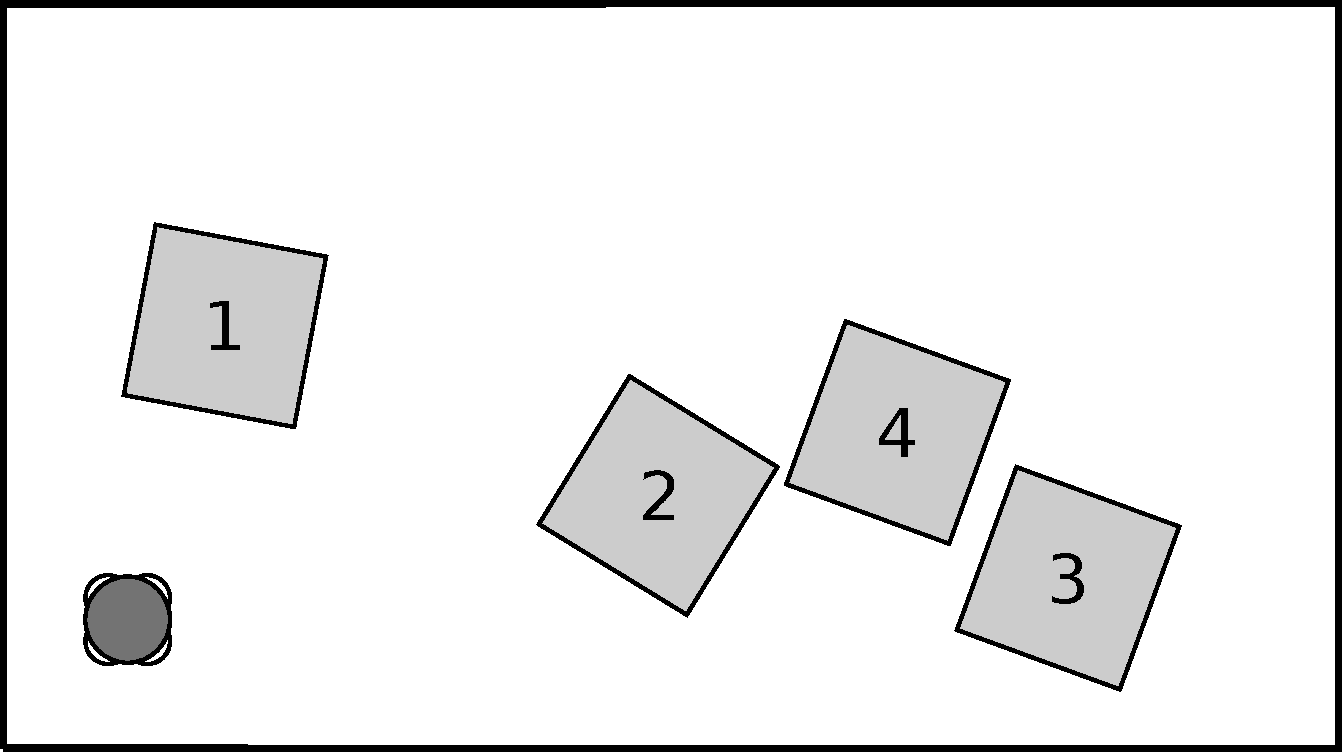
\includegraphics[height=1in]{media_exploration/random_block}
\end{tabular}
\end{center}
\begin{block}{}
 When features are coarse,
 the information content of an unmapped region is not
 always proportional to its size.  
\end{block}
\end{tframe}

\addtocounter{framenumber}{-1}
\begin{tframe}{Obstacle Density Determines Viewpoint}
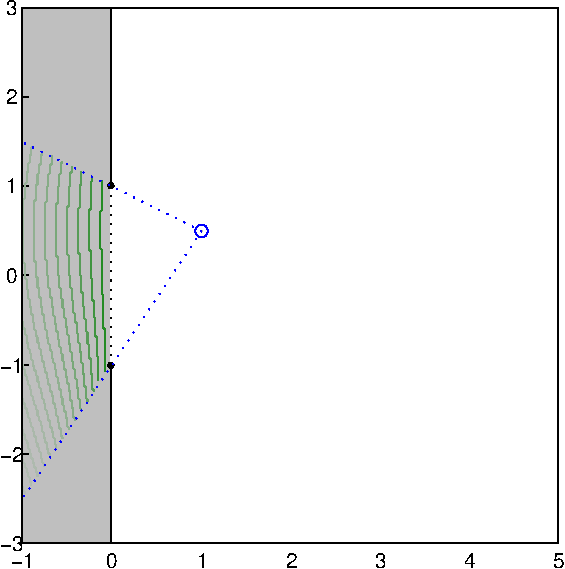
\includegraphics[width=2in]{media_exploration/penetration1}
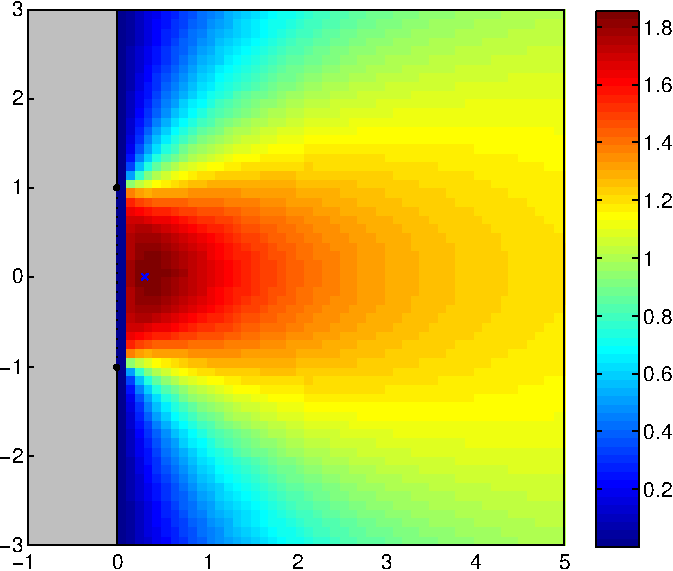
\includegraphics[width=2in]{media_exploration/JEnergy1}
\end{tframe}

\addtocounter{framenumber}{-1}
\begin{tframe}{Obstacle Density Determines Viewpoint}
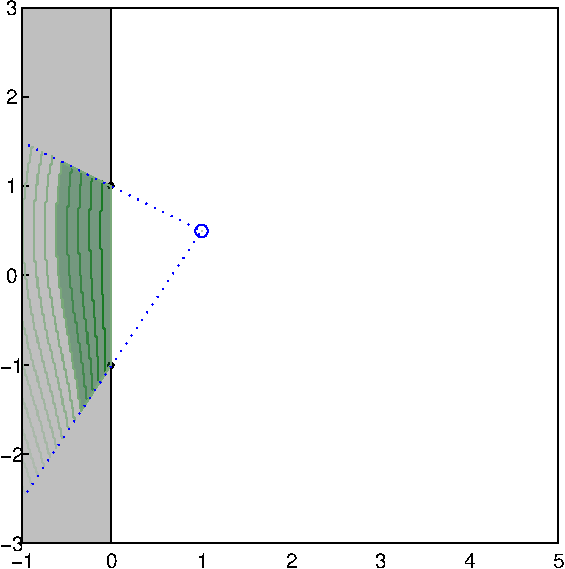
\includegraphics[width=2in]{media_exploration/penetration5}
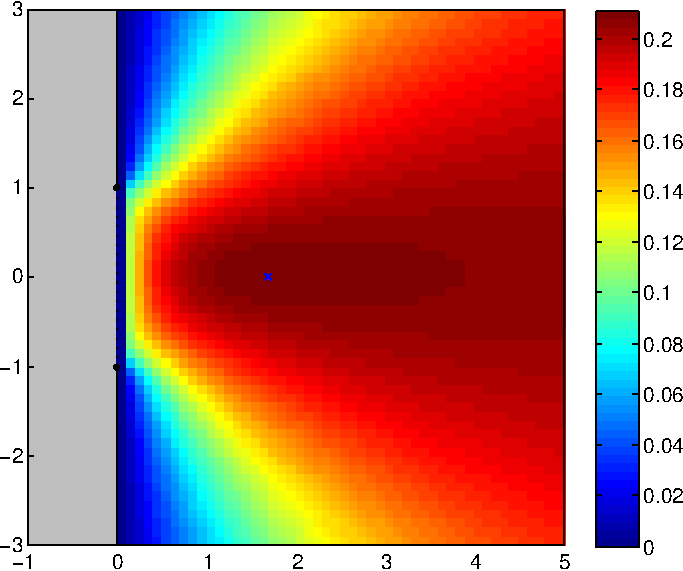
\includegraphics[width=2in]{media_exploration/JEnergy5}
\end{tframe}

\addtocounter{framenumber}{-1}
\begin{tframe}{Obstacle Density Determines Viewpoint}
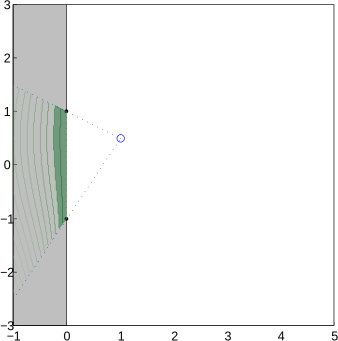
\includegraphics[width=2in]{media_exploration/penetration25}
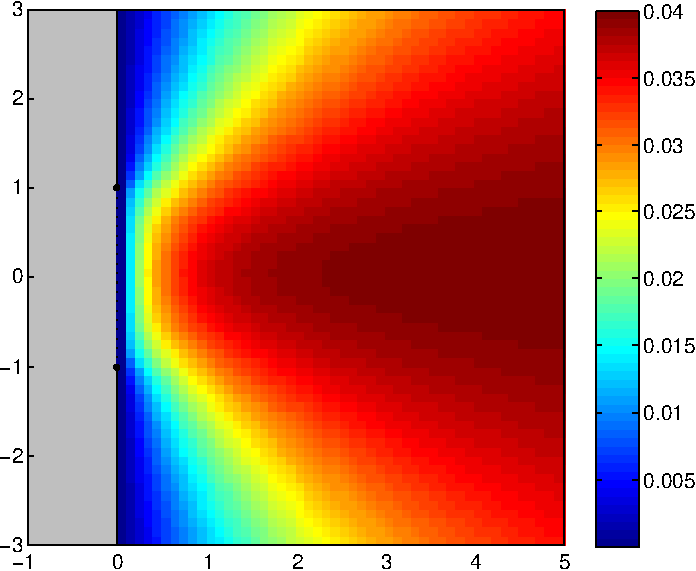
\includegraphics[width=2in]{media_exploration/JEnergy25}
\end{tframe}

\begin{tframe}{Ising-Type Obstacles}
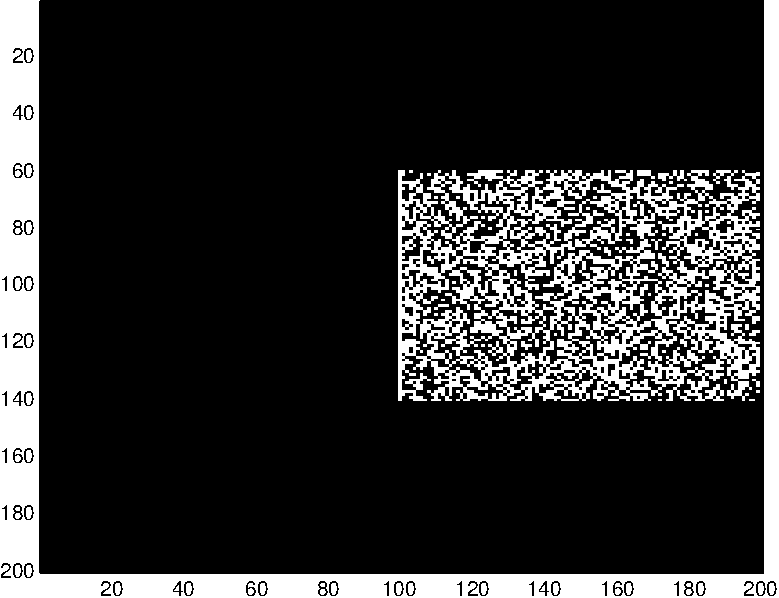
\includegraphics[width=2in]{media_exploration/ising000}
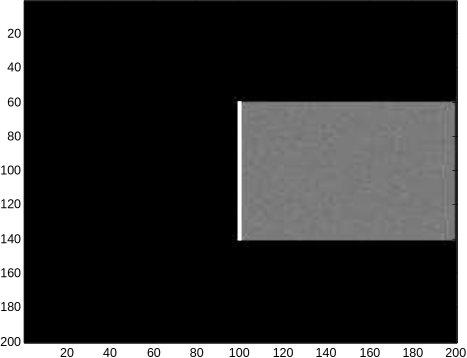
\includegraphics[width=2in]{media_exploration/marg000}

0 Iterations
\end{tframe}

\addtocounter{framenumber}{-1}
\begin{tframe}{Ising-Type Obstacles}
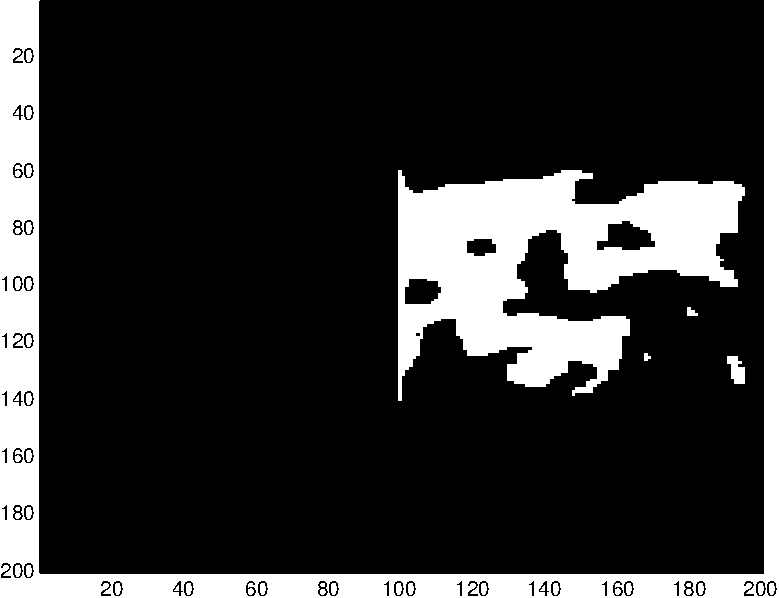
\includegraphics[width=2in]{media_exploration/ising025}
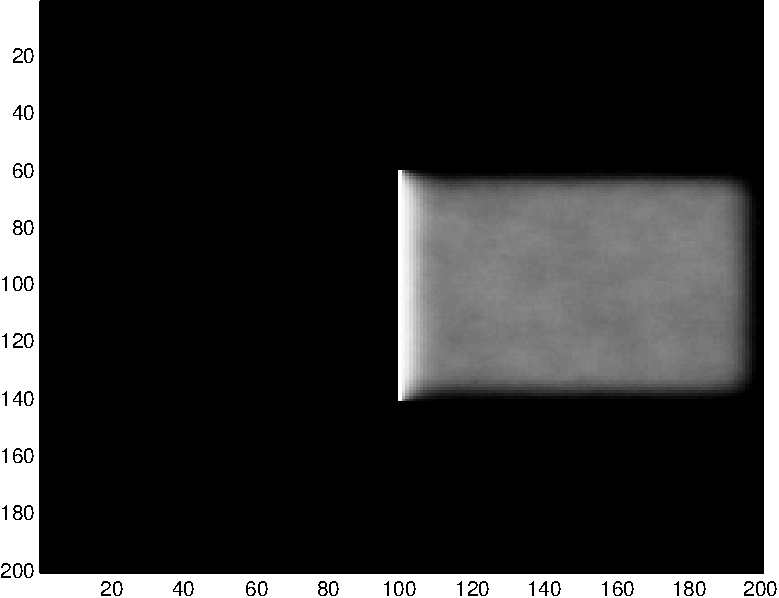
\includegraphics[width=2in]{media_exploration/marg025}

25 Iterations
\end{tframe}

\addtocounter{framenumber}{-1}
\begin{tframe}{Ising-Type Obstacles}
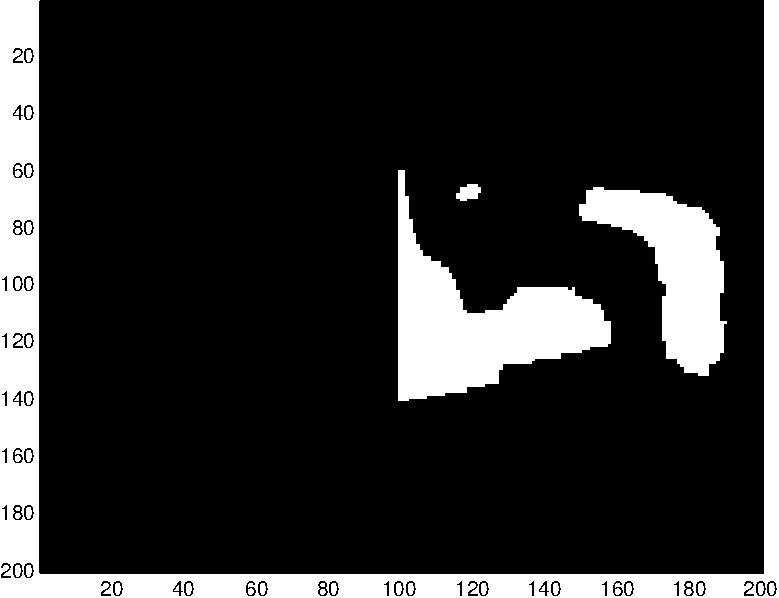
\includegraphics[width=2in]{media_exploration/ising100}
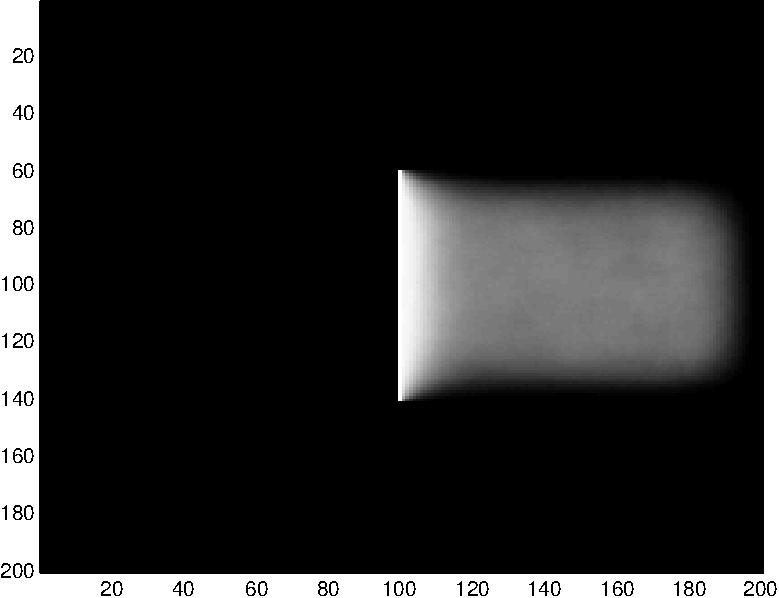
\includegraphics[width=2in]{media_exploration/marg100}

100 Iterations
\end{tframe}

\addtocounter{framenumber}{-1}
\begin{tframe}{Ising-Type Obstacles}
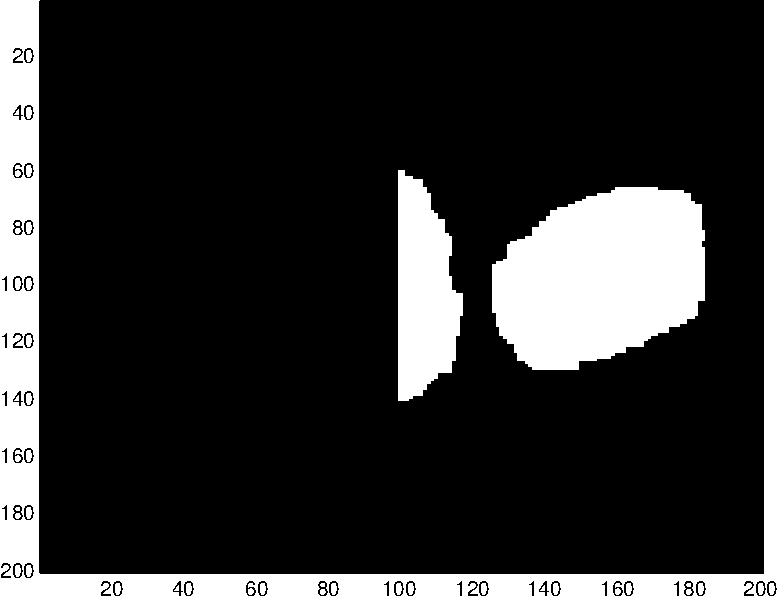
\includegraphics[width=2in]{media_exploration/ising225}
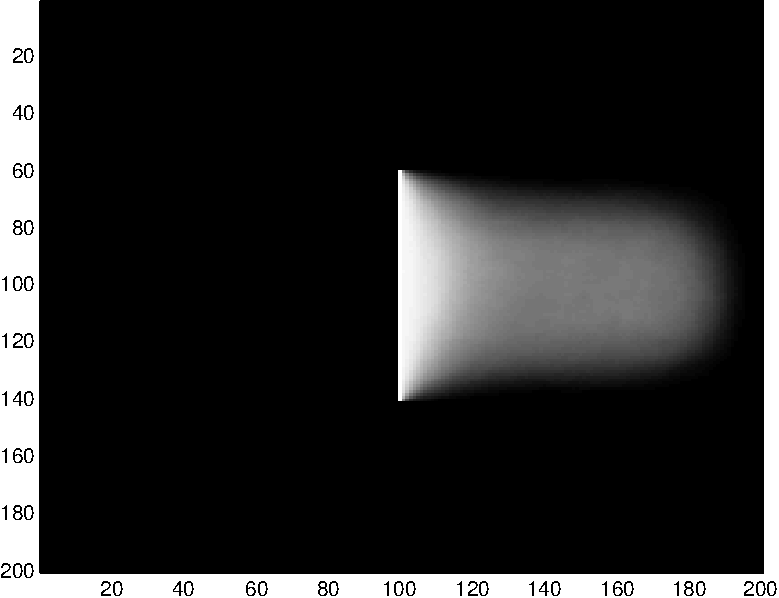
\includegraphics[width=2in]{media_exploration/marg225}

225 Iterations
\end{tframe}

\addtocounter{framenumber}{-1}
\begin{tframe}{Ising-Type Obstacles}
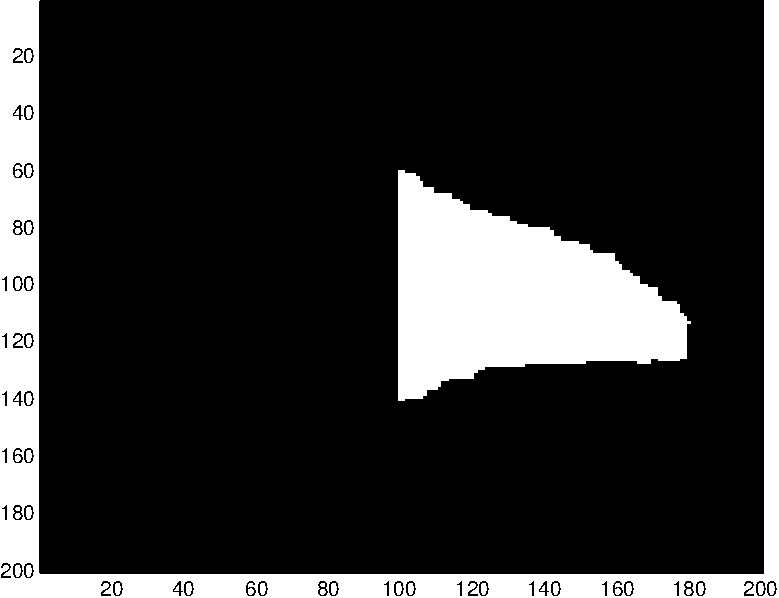
\includegraphics[width=2in]{media_exploration/ising400}
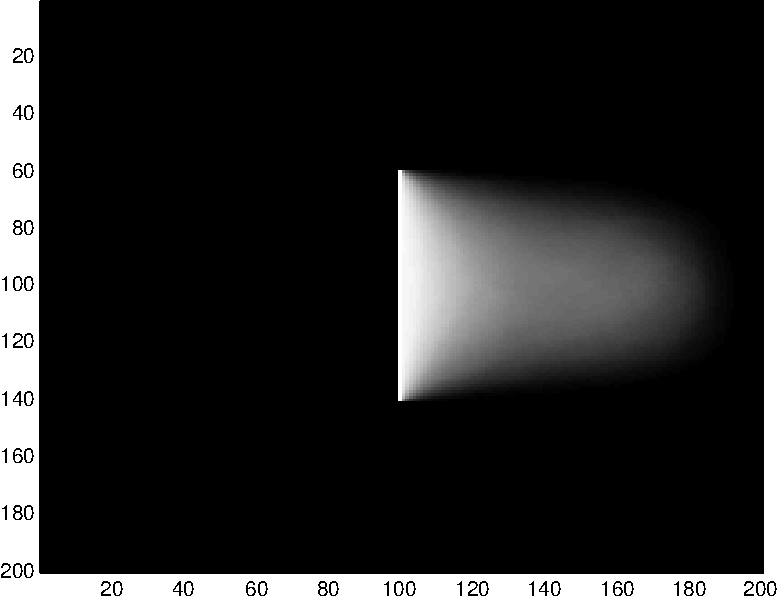
\includegraphics[width=2in]{media_exploration/marg400}

400 Iterations
\end{tframe}

\begin{tframe}{Ising-Type Penetration Profiles}

\bigskip
\begin{center}
\begin{tabular}{ccc}
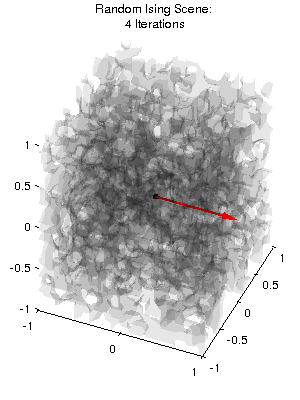
\includegraphics[height=1.2in]{media_exploration/ising_cell_004}&
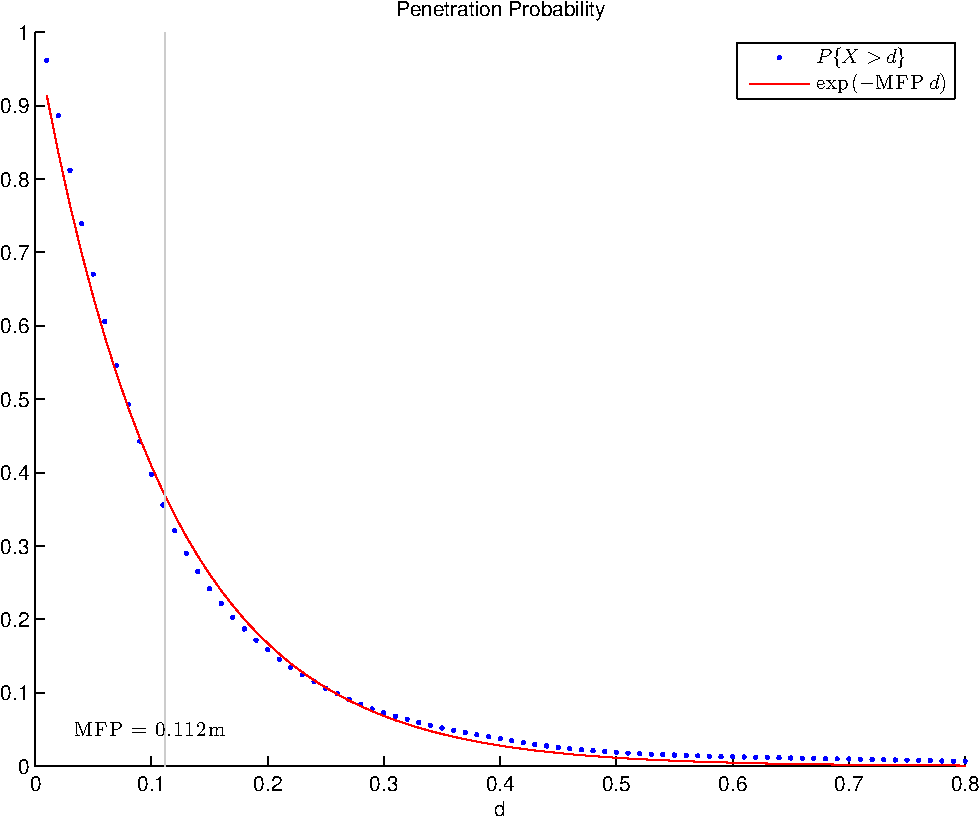
\includegraphics[height=1.2in]{media_exploration/ising_penetration_004}&
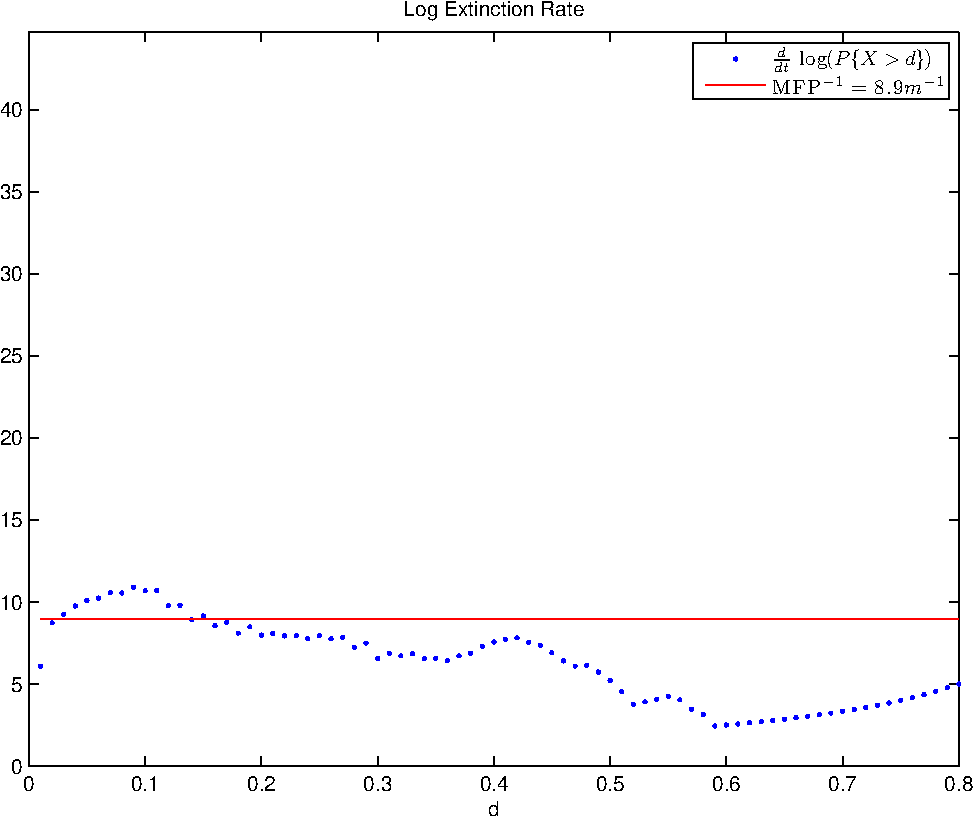
\includegraphics[height=1.2in]{media_exploration/ising_extinction_004}
\end{tabular}
 \end{center}

\bigskip
4 Iterations
\end{tframe}

\addtocounter{framenumber}{-1}
\begin{tframe}{Ising-Type Penetration Profiles}

\bigskip
\begin{center}
\begin{tabular}{ccc}
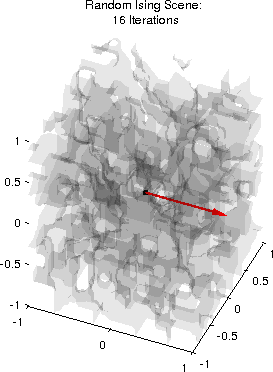
\includegraphics[height=1.2in]{media_exploration/ising_cell_016}&
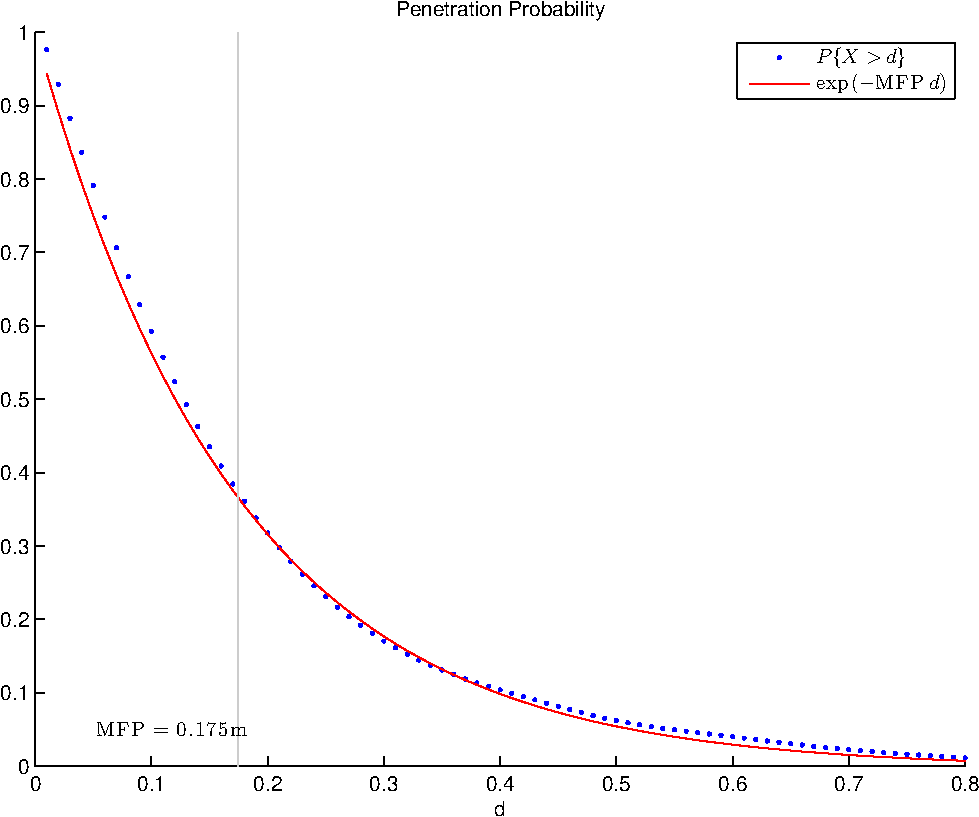
\includegraphics[height=1.2in]{media_exploration/ising_penetration_016}&
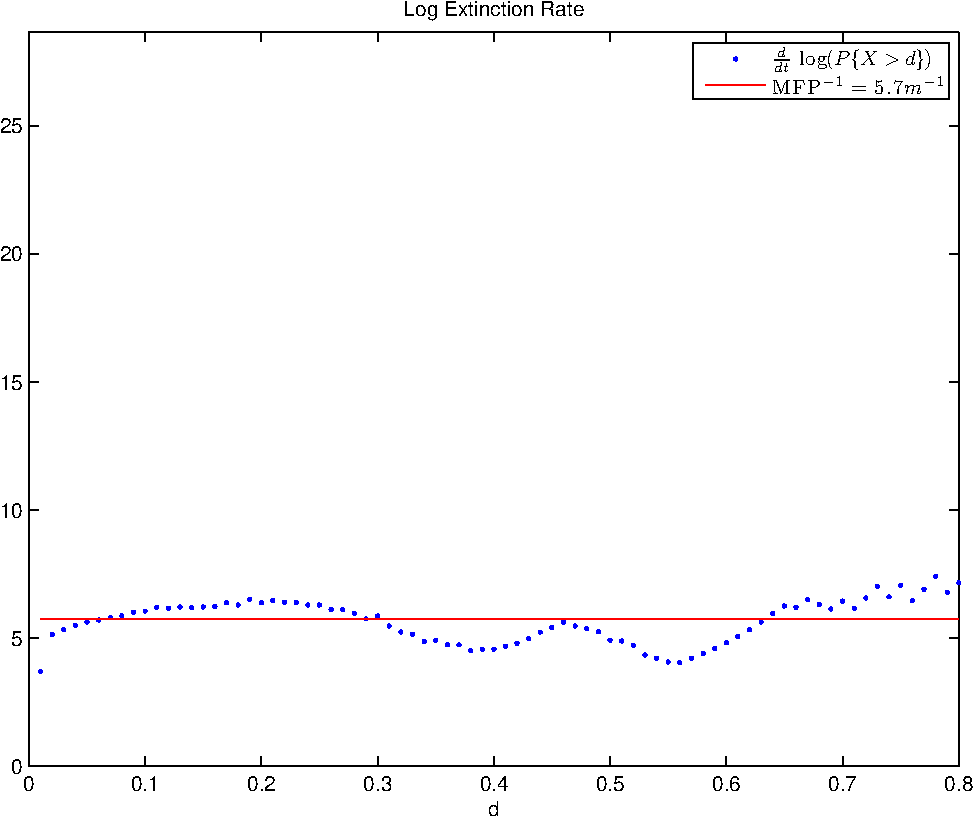
\includegraphics[height=1.2in]{media_exploration/ising_extinction_016}
\end{tabular}
 \end{center}

\bigskip
16 Iterations
\end{tframe}

\addtocounter{framenumber}{-1}
\begin{tframe}{Ising-Type Penetration Profiles}

\bigskip
\begin{center}
\begin{tabular}{ccc}
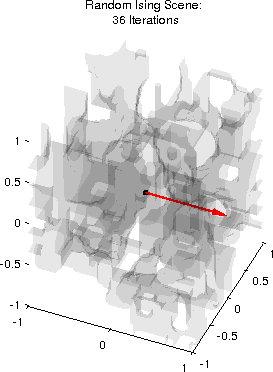
\includegraphics[height=1.2in]{media_exploration/ising_cell_036}&
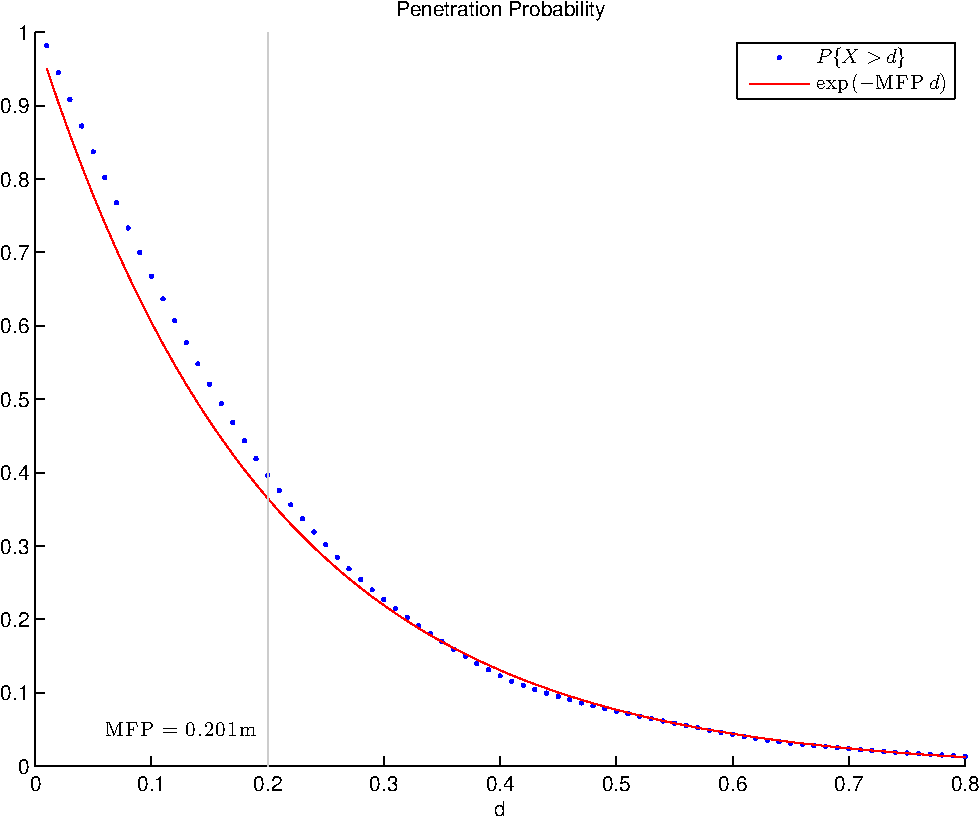
\includegraphics[height=1.2in]{media_exploration/ising_penetration_036}&
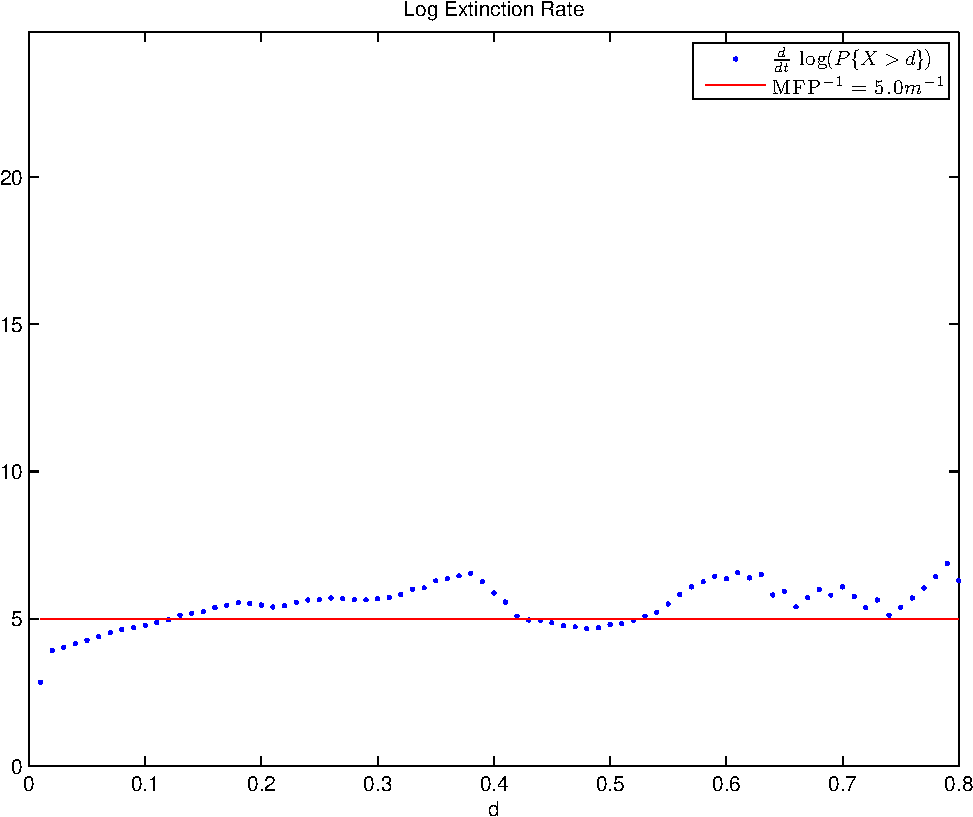
\includegraphics[height=1.2in]{media_exploration/ising_extinction_036}
\end{tabular}
 \end{center}

\bigskip
36 Iterations
\end{tframe}

\begin{tframe}{Ising-Type Penetration Profiles}

\bigskip
\begin{center}
\begin{tabular}{ccc}
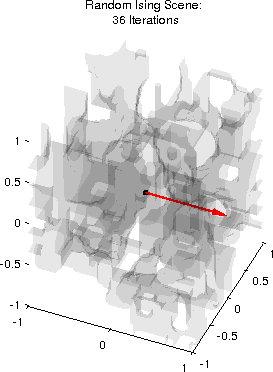
\includegraphics[height=1.2in]{media_exploration/ising_cell_036}&
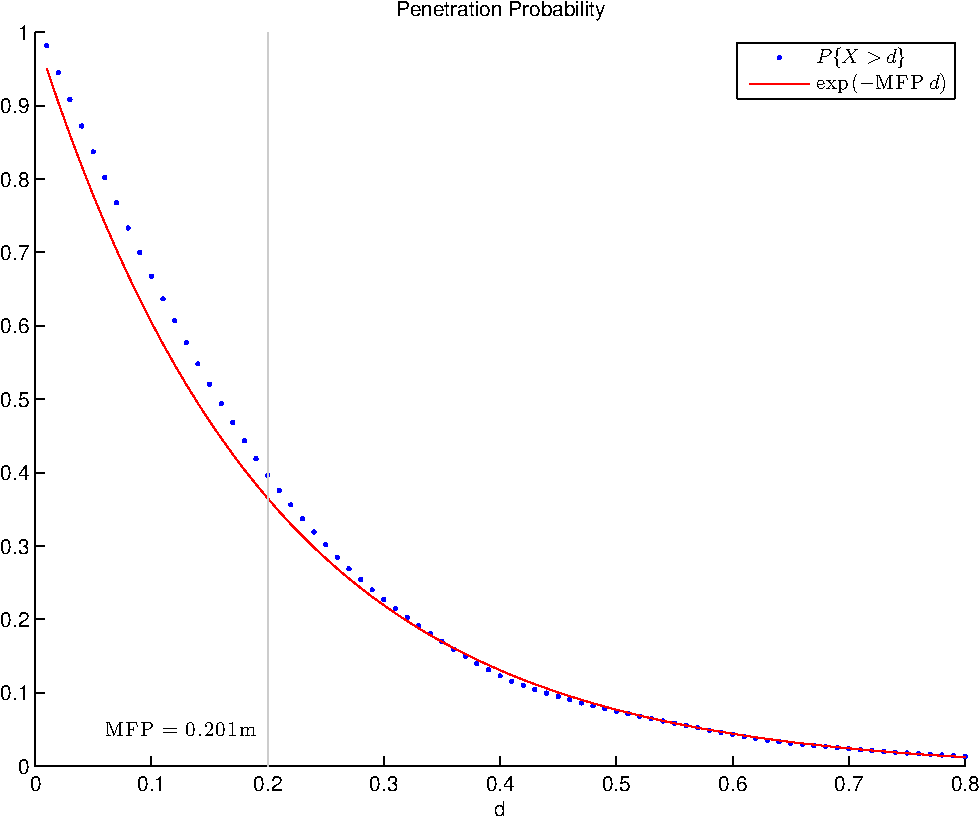
\includegraphics[height=1.2in]{media_exploration/ising_penetration_036}&
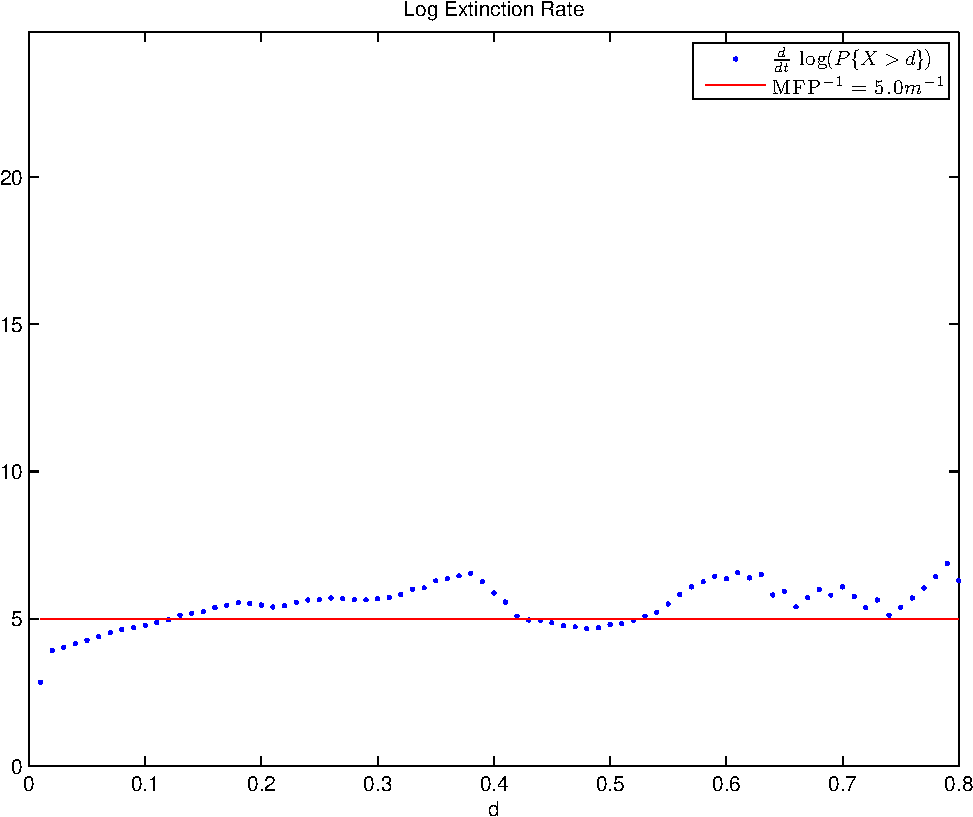
\includegraphics[height=1.2in]{media_exploration/ising_extinction_036}
\end{tabular}
 \end{center}

\bigskip
36 Iterations
\end{tframe}

\begin{tframe}{Information-Seeking Control}

\bigskip
\begin{center}
\begin{tabular}{cc}
\begin{tabular}{c}
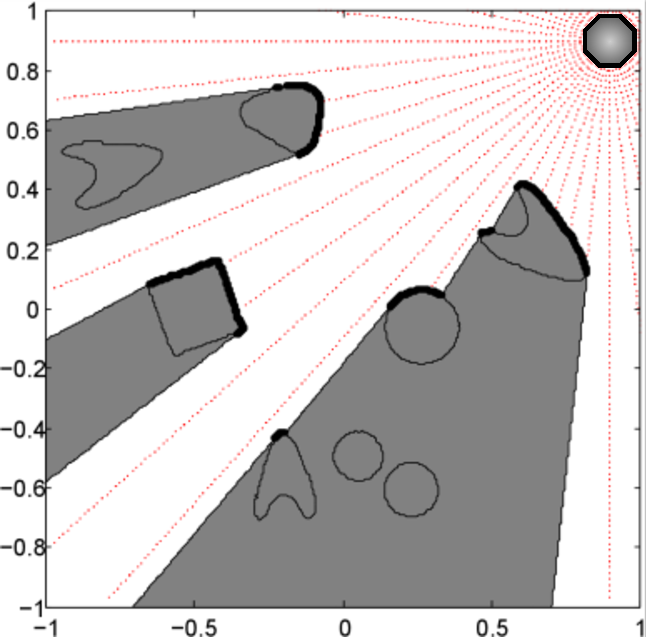
\includegraphics[height=2in]{media_exploration/first_view}
\end{tabular}
&
\parbox[t]{.5\textwidth}{
The information value of a new viewpoint is equal to the uncertainty of
the measurement to be taken there.
}
\end{tabular}
 \end{center}
\end{tframe}

\addtocounter{framenumber}{-1}
\begin{tframe}{Information-Seeking Control}

\bigskip
\begin{center}
\begin{tabular}{cc}
\begin{tabular}{c}
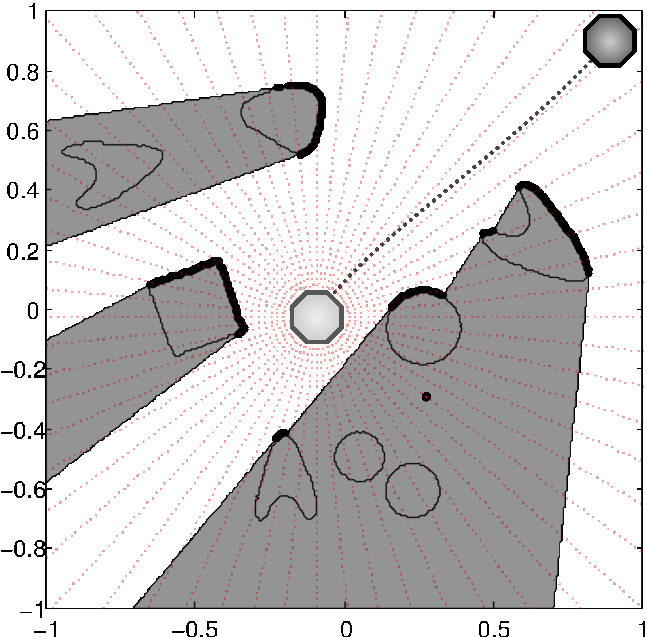
\includegraphics[height=2in]{media_exploration/first_hypoth}
\end{tabular}
&
\parbox[t]{.5\textwidth}{
The information value of a new viewpoint is equal to the uncertainty of
the measurement to be taken there.
}
\end{tabular}
 \end{center}
\end{tframe}

\addtocounter{framenumber}{-1}
\begin{tframe}{Information-Seeking Control}

\bigskip
\begin{center}
\begin{tabular}{cc}
\begin{tabular}{c}
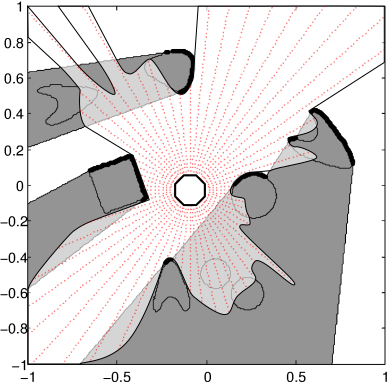
\includegraphics[height=2in]{media_exploration/first_meas}
\end{tabular}
&
\parbox[t]{.5\textwidth}{
The information value of a new viewpoint is equal to the uncertainty of
the measurement to be taken there.
}
\end{tabular}
 \end{center}
\end{tframe}

\begin{tframe}{View Value}
\begin{center}
\begin{align*}
E_t(x) \approx \sum_{ij}& 
\underset{\text{Marginal value of revealing point at $x+g_{ij}$}}
{\underbrace{w_i H(\PP_t[x+g_{ij}\in\A])}}\\
&\qquad\cdot\,
\underset{\text{Probability of revealing point at $x+g_{ij}$}}
{\underbrace{\prod_{i\1<i}\PP_t[x+g_{i\1j}\in\A]^{s/\operatorname{MFP}(x+g_{i\1j})}}}
\end{align*}
where $H(p) = -p\log p - (1-p)\log(1-p)$.
\end{center}
\end{tframe}

\begin{tframe}{Poisson-Voronoi Proxy}
\bigskip
\begin{tabular}{ccc}
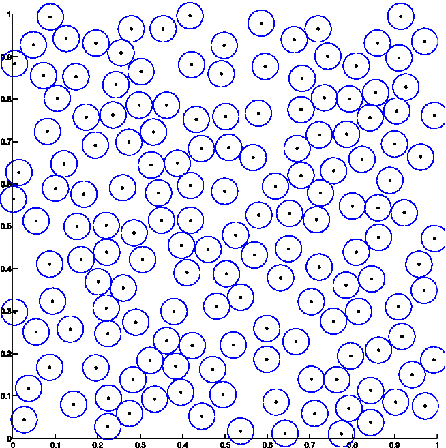
\includegraphics[height=1.2in]{media_exploration/poisson_disk}&
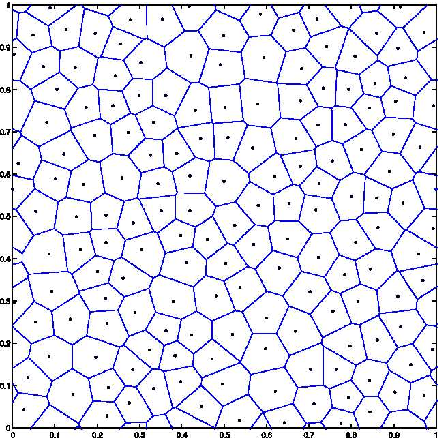
\includegraphics[height=1.1in]{media_exploration/voronoi}&
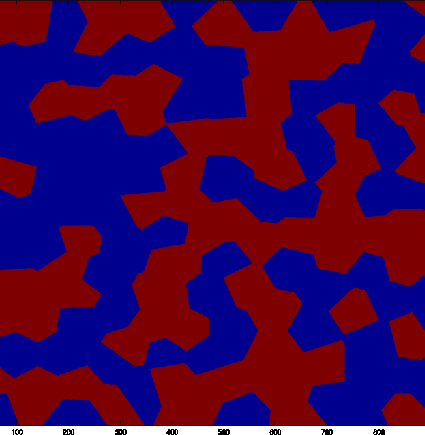
\includegraphics[height=1.3in]{media_exploration/voronoi_chex}\\
Poisson-Disk Sampling &
Voronoi Tesselation &
Voronoi Checkerboard
\end{tabular}
\end{tframe}

\begin{tframe}{Poisson-Voronoi Proxy}
\begin{center}
\begin{tabular}{c}
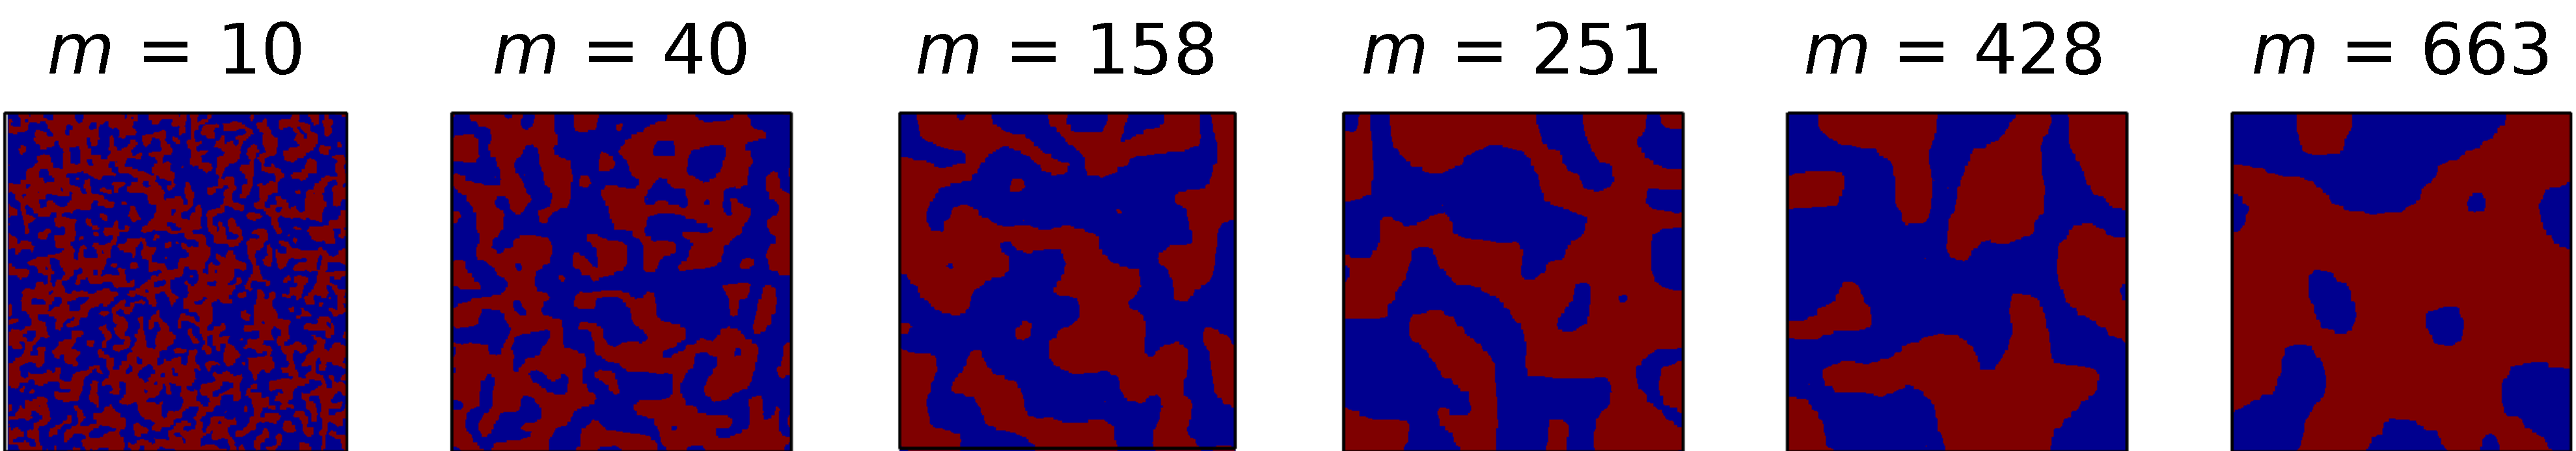
\includegraphics[width=4in]{media_exploration/entropy_ising}\\
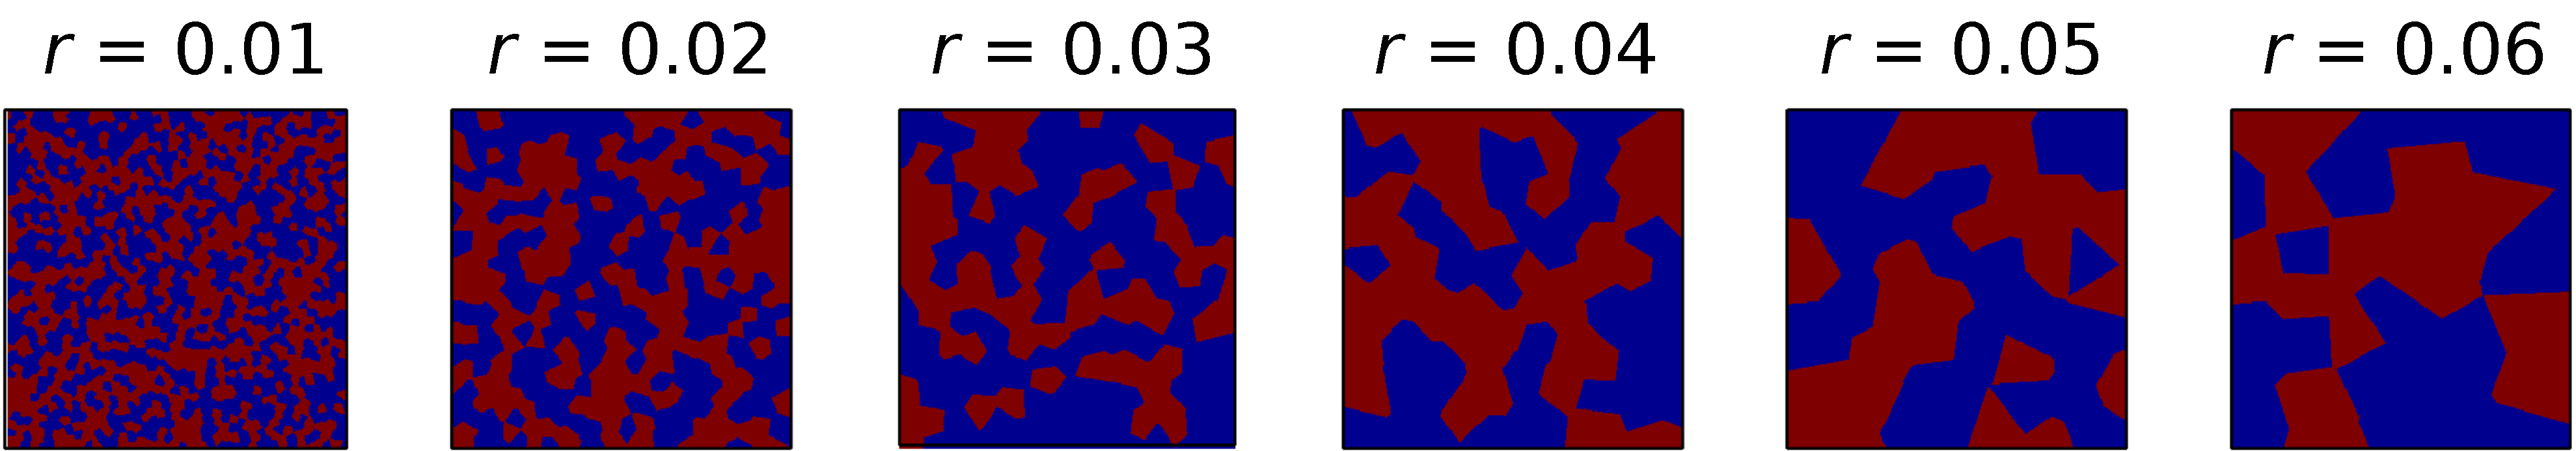
\includegraphics[width=4in]{media_exploration/entropy_chex}
\end{tabular}
\end{center}
\end{tframe}

\begin{tframe}{Poisson-Voronoi Proxy}

\bigskip
\begin{tabular}{ccc}
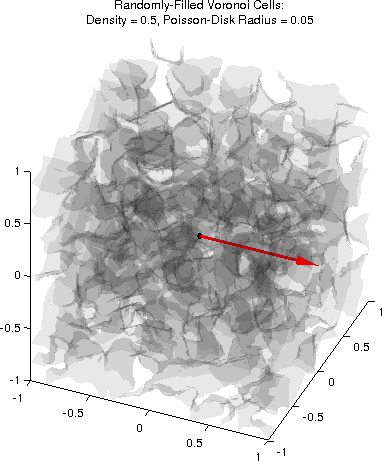
\includegraphics[height=1.2in]{media_exploration/cell_05}&
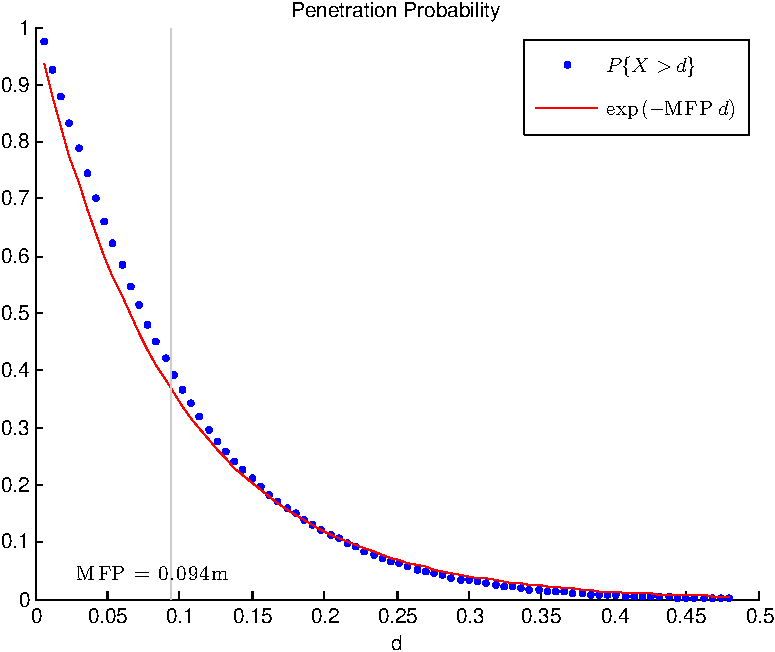
\includegraphics[height=1.2in]{media_exploration/penetration_05}&
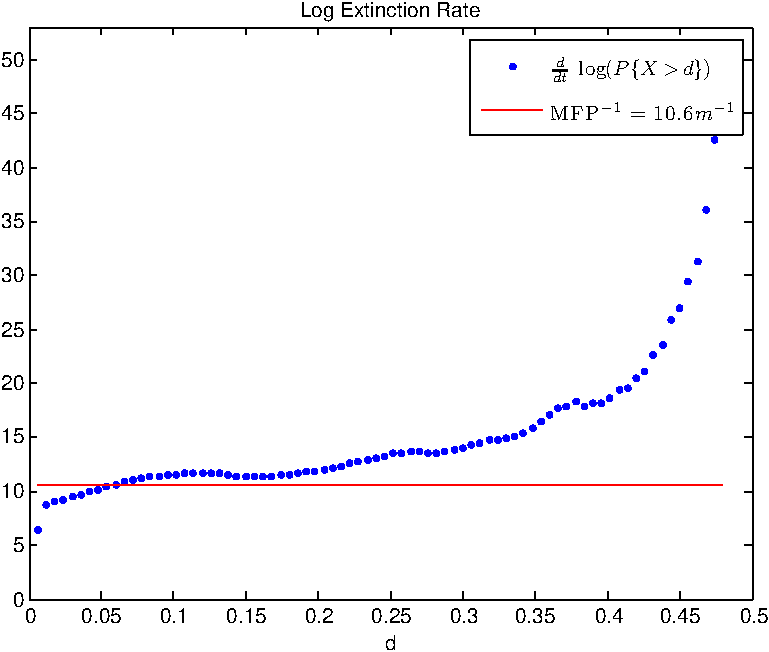
\includegraphics[height=1.2in]{media_exploration/extinction_05}
\end{tabular}

Mean free path scales directly with Poisson-disc radius,
so this needs to be computed only once
\end{tframe}


\begin{tframe}{Computing Graph Weights $w_i$}

\bigskip
\begin{center}
\begin{tabular}{cc}
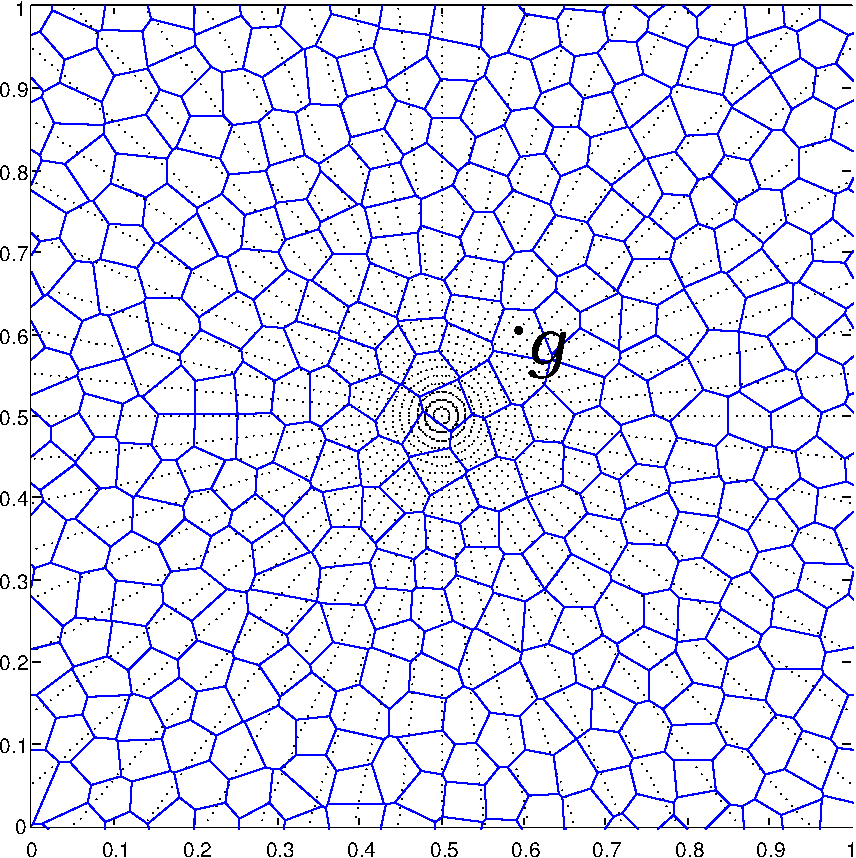
\includegraphics[height=1.5in]{media_exploration/voronoi_grid}&
\phantom{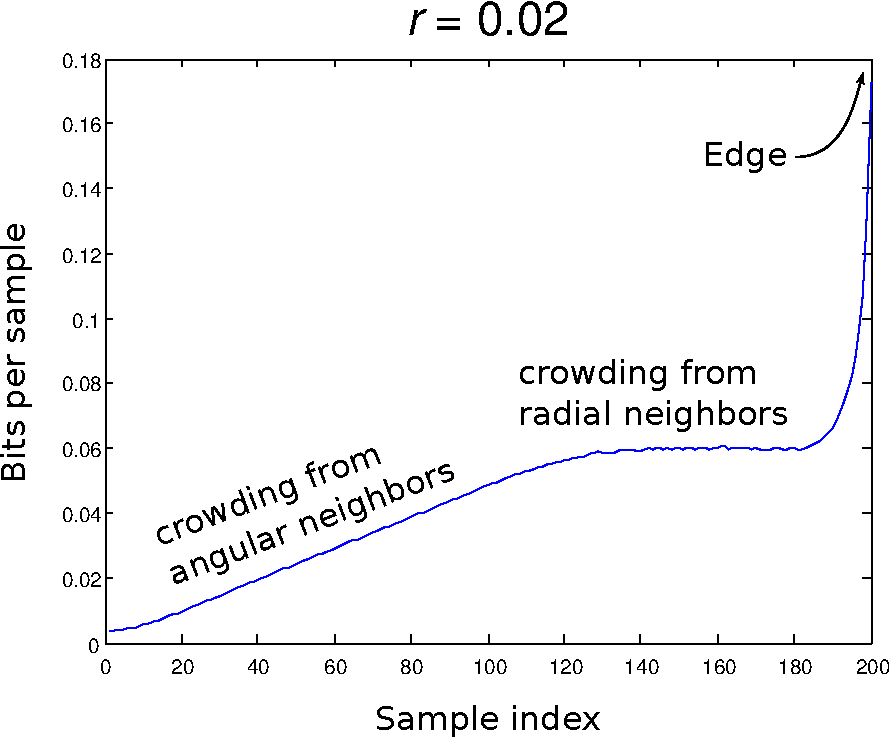
\includegraphics[height=1.5in]{media_exploration/weight_profile}}
\end{tabular}
\end{center}
\end{tframe}

\addtocounter{framenumber}{-1}
\begin{tframe}{Computing Graph Weights $w_i$}

\bigskip
\begin{center}
\begin{tabular}{cc}
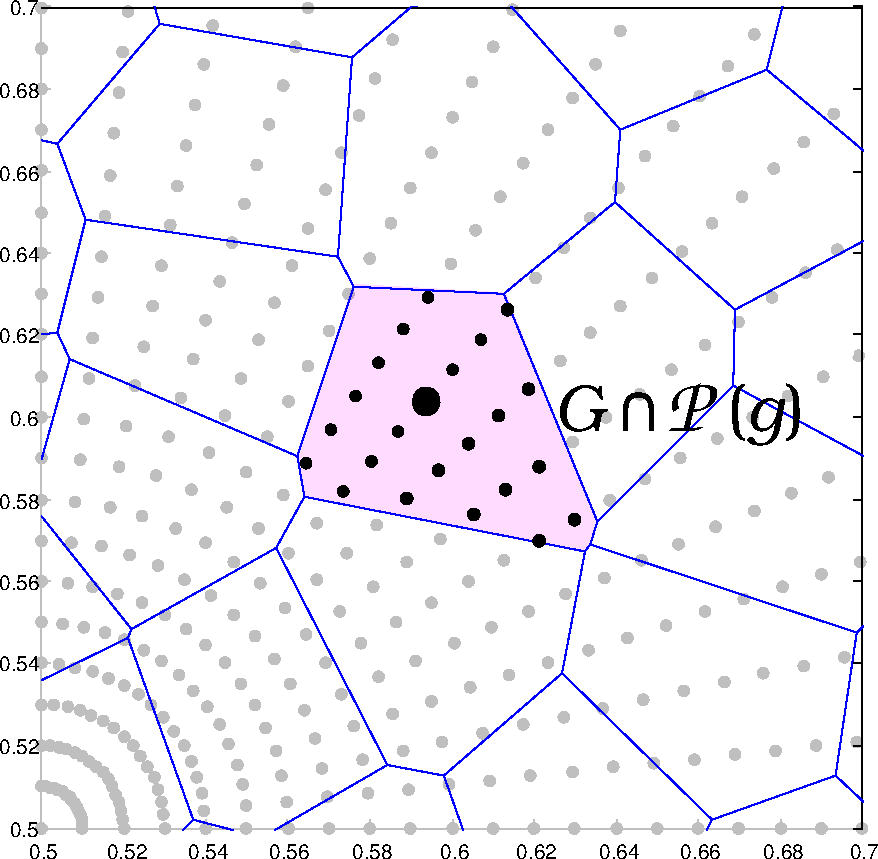
\includegraphics[height=1.5in]{media_exploration/voronoi_grid_closeup}&
\visible<2>{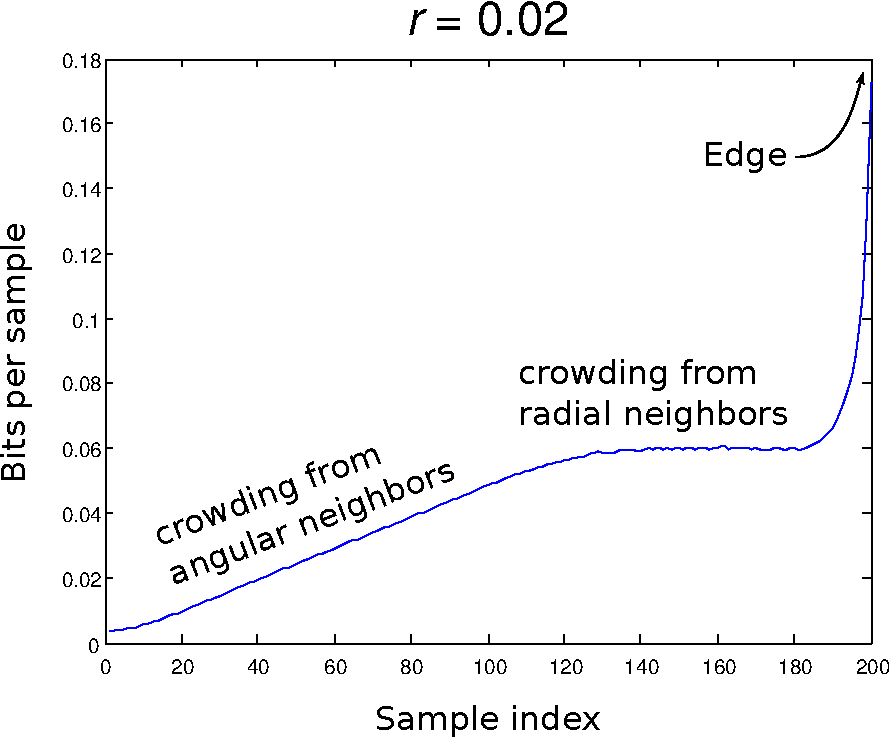
\includegraphics[height=1.5in]{media_exploration/weight_profile}}
\end{tabular}
\end{center}
\end{tframe}

\begin{tframe}{Computing Graph Weights $w_i$}

\bigskip
\begin{center}
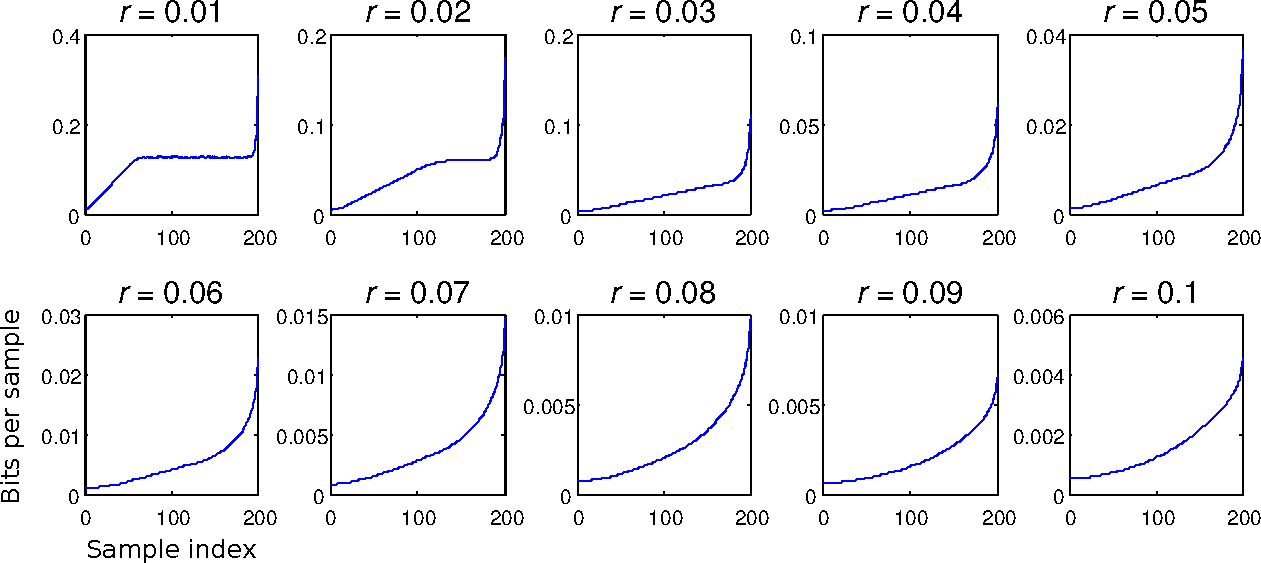
\includegraphics[width=4in]{media_exploration/weight_profiles}
\end{center}
\end{tframe}

\begin{tframe}{3D Graph Weights}
\begin{center}
\begin{tabular}{cc}
\begin{tabular}{c}
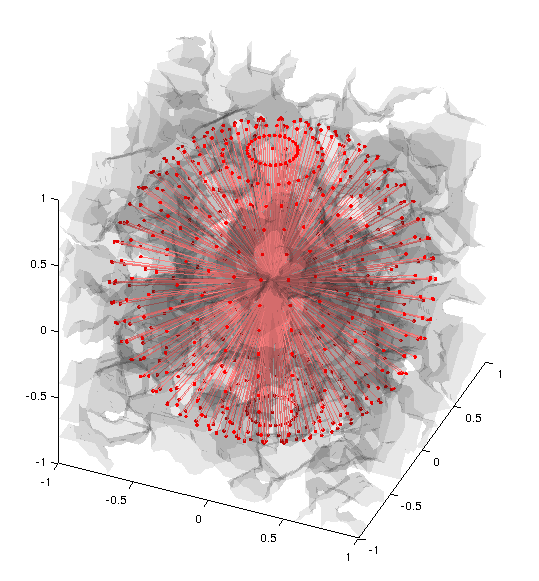
\includegraphics[height=1.5in]{media_exploration/samples.png}
\end{tabular}&
\begin{tabular}{cc}
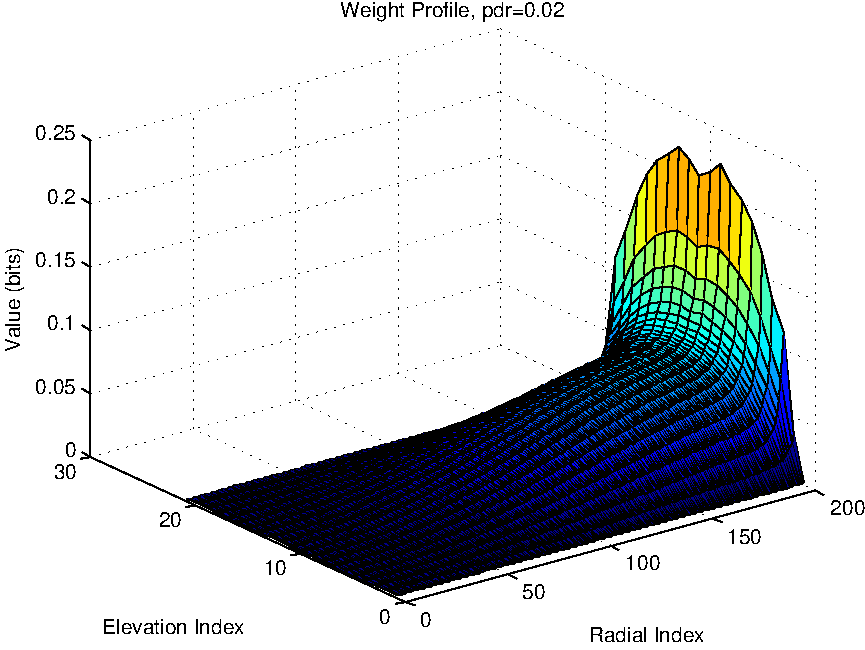
\includegraphics[width=1in]{media_exploration/W02}&
\includegraphics[width=1in]{media_exploration/W04}\\
\includegraphics[width=1in]{media_exploration/W06}&
\includegraphics[width=1in]{media_exploration/W08}
\end{tabular}
\end{tabular}
\end{center}
\end{tframe}

\begin{tframe}{2D Exploration}
\begin{center}

\bigskip
\begin{tabular}{ccc}
\includegraphics[width=1.2in]{media_exploration/2D_scene_01}&
\includegraphics[width=1.2in]{media_exploration/2D_marginal_01}&
\includegraphics[width=1.2in]{media_exploration/2D_energy_01}
\\ Visibility & Marginals & View Value
\end{tabular}
\end{center}
\end{tframe}

\addtocounter{framenumber}{-1}
\begin{tframe}{2D Exploration}
\begin{center}

\bigskip
\begin{tabular}{ccc}
\includegraphics[width=1.2in]{media_exploration/2D_scene_02}&
\includegraphics[width=1.2in]{media_exploration/2D_marginal_02}&
\includegraphics[width=1.2in]{media_exploration/2D_energy_02}
\\ Visibility & Marginals & View Value
\end{tabular}
\end{center}
\end{tframe}

\addtocounter{framenumber}{-1}
\begin{tframe}{2D Exploration}
\begin{center}

\bigskip
\begin{tabular}{ccc}
\includegraphics[width=1.2in]{media_exploration/2D_scene_03}&
\includegraphics[width=1.2in]{media_exploration/2D_marginal_03}&
\includegraphics[width=1.2in]{media_exploration/2D_energy_03}
\\ Visibility & Marginals & View Value
\end{tabular}
\end{center}
\end{tframe}

\addtocounter{framenumber}{-1}
\begin{tframe}{2D Exploration}
\begin{center}

\bigskip
\begin{tabular}{ccc}
\includegraphics[width=1.2in]{media_exploration/2D_scene_04}&
\includegraphics[width=1.2in]{media_exploration/2D_marginal_04}&
\includegraphics[width=1.2in]{media_exploration/2D_energy_04}
\\ Visibility & Marginals & View Value
\end{tabular}
\end{center}
\end{tframe}

\addtocounter{framenumber}{-1}
\begin{tframe}{2D Exploration}
\begin{center}

\bigskip
\begin{tabular}{ccc}
\includegraphics[width=1.2in]{media_exploration/2D_scene_05}&
\includegraphics[width=1.2in]{media_exploration/2D_marginal_05}&
\includegraphics[width=1.2in]{media_exploration/2D_energy_05}
\\ Visibility & Marginals & View Value
\end{tabular}
\end{center}
\end{tframe}

\begin{tframe}{3D Exploration}
\begin{center}

\bigskip
\begin{tabular}{ccc}
\includegraphics[width=1.2in]{media_exploration/view_01}&
\includegraphics[width=1.2in]{media_exploration/marginal_01}&
\includegraphics[width=1.2in]{media_exploration/energy_01}
\\ Visibility & Marginals & View Value
\end{tabular}
\end{center}
\end{tframe}

\addtocounter{framenumber}{-1}
\begin{tframe}{3D Exploration}
\begin{center}

\bigskip
\begin{tabular}{ccc}
\includegraphics[width=1.2in]{media_exploration/view_02}&
\includegraphics[width=1.2in]{media_exploration/marginal_02}&
\includegraphics[width=1.2in]{media_exploration/energy_02}
\\ Visibility & Marginals & View Value
\end{tabular}
\end{center}
\end{tframe}

\addtocounter{framenumber}{-1}
\begin{tframe}{3D Exploration}
\begin{center}

\bigskip
\begin{tabular}{ccc}
\includegraphics[width=1.2in]{media_exploration/view_03}&
\includegraphics[width=1.2in]{media_exploration/marginal_03}&
\includegraphics[width=1.2in]{media_exploration/energy_03}
\\ Visibility & Marginals & View Value
\end{tabular}
\end{center}
\end{tframe}

\addtocounter{framenumber}{-1}
\begin{tframe}{3D Exploration}
\begin{center}

\bigskip
\begin{tabular}{ccc}
\includegraphics[width=1.2in]{media_exploration/view_04}&
\includegraphics[width=1.2in]{media_exploration/marginal_04}&
\includegraphics[width=1.2in]{media_exploration/energy_04}
\\ Visibility & Marginals & View Value
\end{tabular}
\end{center}
\end{tframe}

\addtocounter{framenumber}{-1}
\begin{tframe}{3D Exploration}
\begin{center}

\bigskip
\begin{tabular}{ccc}
\includegraphics[width=1.2in]{media_exploration/view_05}&
\includegraphics[width=1.2in]{media_exploration/marginal_05}&
\includegraphics[width=1.2in]{media_exploration/energy_05}
\\ Visibility & Marginals & View Value
\end{tabular}
\end{center}
\end{tframe}

\begin{tframe}{Comparisons}
\begin{center}
\begin{tabular}{c}
\includegraphics[width=4in]{media_exploration/simple_cropped}\\
\includegraphics[width=4in]{media_exploration/ising_cropped}
\end{tabular}
\end{center}
\end{tframe}

\begin{tframe}{Speedup: Parallel Bits}

\bigskip
\begin{center}
\begin{tabular}{cc}
\includegraphics[height=1.4in]{media_exploration/iso-01}&
\includegraphics[height=1.4in]{media_exploration/par000}
\end{tabular}
\end{center}
\end{tframe}

\addtocounter{framenumber}{-1}
\begin{tframe}{Speedup: Parallel Bits}

\bigskip
\begin{center}
\begin{tabular}{cc}
\includegraphics[height=1.4in]{media_exploration/iso-02}&
\includegraphics[height=1.4in]{media_exploration/par025}
\end{tabular}
\end{center}
\end{tframe}

\addtocounter{framenumber}{-1}
\begin{tframe}{Speedup: Parallel Bits}

\bigskip
\begin{center}
\begin{tabular}{cc}
\includegraphics[height=1.4in]{media_exploration/iso-03}&
\includegraphics[height=1.4in]{media_exploration/par100}
\end{tabular}
\end{center}
\end{tframe}

\addtocounter{framenumber}{-1}
\begin{tframe}{Speedup: Parallel Bits}

\bigskip
\begin{center}
\begin{tabular}{cc}
\includegraphics[height=1.4in]{media_exploration/iso-04}&
\includegraphics[height=1.4in]{media_exploration/par225}
\end{tabular}
\end{center}
\end{tframe}

\begin{tframe}{Anisotropic Prior}

\bigskip
\begin{center}
\begin{tabular}{cc}
\includegraphics[height=1.7in]{media_exploration/angly}&
\includegraphics[height=1.7in]{media_exploration/frame_179}
\end{tabular}
\end{center}
\end{tframe}

\begin{tframe}{Extending the Horizon}
\begin{center}

\bigskip
\begin{tabular}{ccc}
\includegraphics[width=1.3in]{media_exploration/extra/marg}&
\includegraphics[width=1.3in]{media_exploration/extra/sim_matrix}&
\includegraphics[width=1.3in]{media_exploration/extra/10samples}
\end{tabular}
\end{center}
\end{tframe}

\begin{tframe}{Contribution}
 \begin{itemize}
  \item First bounds on indistinguishable set with IMU bias drift.
  \item Developed system for video segmentation leveraging image-plane segmentations.
  \item Developed an algorithm for in-place state reduction. Related POMDP to large body of ancient (pre-1980) research in digital circuit optimization.
  \item Developed an algorithm for efficient exploration of unknown scenes with nontrivial topology
 \end{itemize}
\end{tframe}
